\section{Build structure}
\label{Sprint2_buildstructure}
\textit{In this section all the dependencies between apps and libraries are described, with the goal of finding out what is needed to get the apps to run and which dependencies would have to be removed to be able to make apps standalone.}

\subsection{Motivation}

When the 2nd sprint started, the apps and libraries recursively downloaded and build all the libraries they were dependent on. This resulted in having large projects, since many libraries occurred multiple times in one project. The graph in Figure \ref{oldbuild} shows the build tree for the app ‘Sequence’. As seen from the graph the library ‘local-db’ is build 16 times before the Sequence app itself is build. All in all the entire project for Sequence had to build 31 libraries before it could build the app. Which took a lot of time on the build server.

\begin{figure}[H]
	\centering
	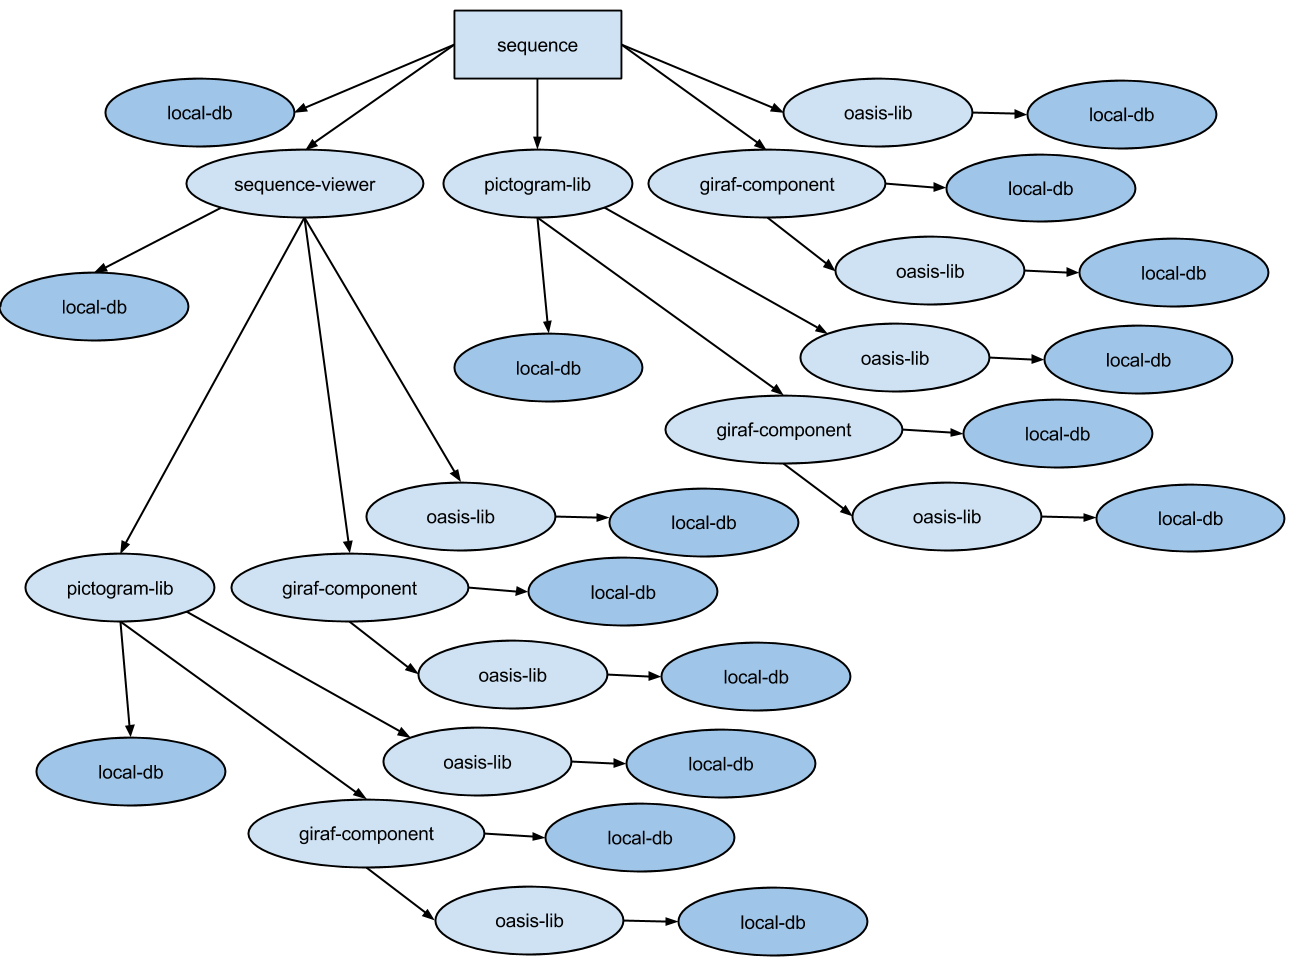
\includegraphics[width=0.8 \textwidth]{pictures/oldbuild.png}
	\caption{Build tree for old Sequence}
	\label{oldbuild}
\end{figure}

\subsection{Android archive}
As an solution, we want each libraries to build a library file, which can be used in multiple places. This reduces the build time of all the projects since the apps or libraries just need to download the prebuilt library files.
This is where Android archive (AAR) files are introduced. AAR files are binary distributions of an Android Library Project, which works like a standard Java jar library. The difference between a jar library and an aar library is that the aar library includes resources, which allows for visual components like an login screen, which can then be used across multiple applications. 
The distribution of libraries (aar) and apps will be explained in Section x.x (reference to collaboration chapter), since more groups were involved in making this happen.

\subsection{Solution}
By using a pre-built library, each application only has to build itself with the libraries include in the application as shown in the the graph in Figure \ref{newbuild}. It is important to know that all libraries included in other libraries have to be included by the app. It means that even if the ‘Sequence’ app didn't use ‘oasis-lib’ directly, it would still have to include it because ‘giraf-component’ is using it.

\begin{figure}[H]
	\centering
	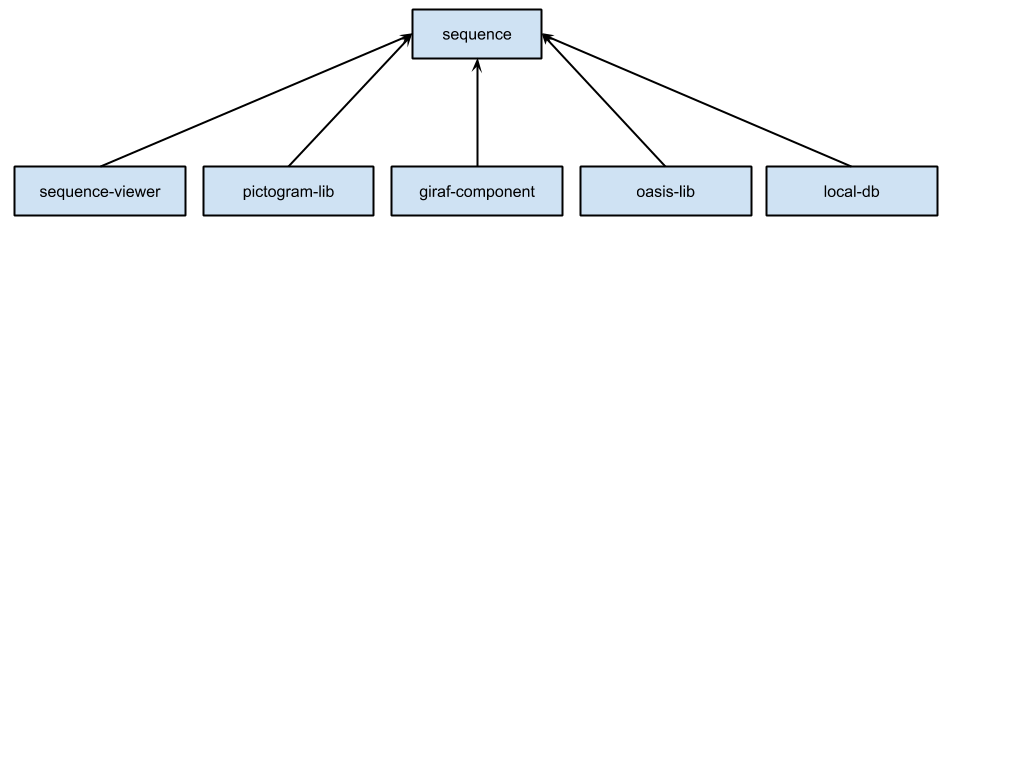
\includegraphics[width=0.8 \textwidth]{pictures/newbuild.png}
	\caption{Build tree for new Sequence}
	\label{newbuild}
\end{figure}

Before implementing this solution, libraries could occur a number of times equal to 1, for the app, plus the number of libraries already present. I.e ‘Sequence’ adds the library ‘sequence-viewer’, then ‘pictogram-lib’, then ‘giraf-component’, then ‘oasis-lib’, and then lastly ‘localdb’ is added.  Figure x.x is the visual representation of this. As it can be seen the number of builds follow an arithmetic series on the form:


\begin{center}
	$1 lib_{1} + 2 lib_{2} + 4 lib_{3} + 8 lib_{4} + 16 lib_{5}$	
\end{center}


This can be summarized to:

\begin{center}
    $\displaystyle\sum_{i=0}^{i<n} 2^n$
\end{center}



Where n is the number of different libraries added to the app.

This is a worst case scenario but as it can be seen from Section “ref til dependencies” most apps were in a worst case state before the change.
After implementing the solution, the total number of library-builds has been reduced to just one per different library. This means that after the change there is a linear growth between the number of libraries and the number of library-builds.

As it can be seen from Table x.x, our solution reduced the number of libraries being build drastically, which in turn reduced the build time for each app on Jenkins by a detectable margin.

\begin{table}[H]
	\centering
	\begin{tabularx}{\textwidth}{>{\raggedright}Xp{\textwidth/3}p{\textwidth/3}}
		 & \textbf{Before} & \textbf{After} \\ \noalign{\vskip 2mm}
		\hline \textbf{Formula}: & $\displaystyle\sum_{i=0}^{i<n} 2^n$ & n \\ \noalign{\vskip 2mm}
		\hline \textbf{Launcher}: & 8 & 4 \\ \noalign{\vskip 2mm}
		\hline \textbf{Sequence}: & 31 & 5 \\ \noalign{\vskip 2mm}
		\hline \textbf{Timer}: & 18 & 7 \\ \noalign{\vskip 2mm}
		\hline \textbf{Pictocreator}: & 15 & 4 \\ \noalign{\vskip 2mm}
		\hline \textbf{Categorymanager}: & 17 & 6 \\ \noalign{\vskip 2mm}
		\hline \textbf{Pictosearch}: & 7 & 3 \\ \noalign{\vskip 2mm}
		\hline \textbf{Voicegame}: & 7 & 3 \\ \noalign{\vskip 2mm}
		\hline \textbf{Categorygame}: & 15 & 4 \\ \noalign{\vskip 2mm}
		\hline \textbf{Pictoreader}: & 17 & 6 \\ \noalign{\vskip 2mm}
		\hline \textbf{Lifestories}: & 31 & 5 \\ \noalign{\vskip 2mm}
		\hline \textbf{Weekschedule}: & 15 & 4 \\ \noalign{\vskip 2mm}
		\hline \textbf{Administration}: & 7 & 3 \\ \noalign{\vskip 2mm}
		\hline
		
	\end{tabularx}
	\label{test}
	\caption{List of apps and libraries}
\end{table}
